\documentclass{beamer}

\setlength{\parskip}{\baselineskip}
\setlength{\parindent}{0pt}

%\usepackage{fontawesome}
\usepackage{default}
\usepackage{tabularx}
\usepackage{url}
\usepackage{graphicx}
\usepackage{color}


\title{\huge{SIAM Student Chapter at TU Delft}}
\author{Reinaldo Astudillo, Manuel Baumann, Thea Vuik}
\titlegraphic{\vspace{-0.3cm}
\includegraphics[scale=0.14]{SSC_Delft_new}}
\date{\footnotesize{September 19, 2014}}

\begin{document}

\frame{\titlepage}
\begin{frame}
\frametitle{What's a SIAM student chapter?}
\begin{columns}
 \begin{column}{0.7\textwidth}
 \begin{itemize}
  \item SIAM is the biggest horizontal organization in Applied Mathematics,
  \item Students chapters exist in 105 universities (only a few in Europe),
  \item at TU Delft: Connect PhD students from all departments.
 \end{itemize}

 \end{column}

 \begin{column}{0.4\textwidth}
  \begin{figure}[t]
  \centering
  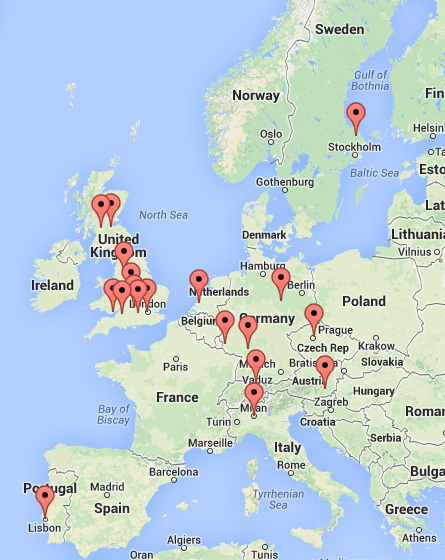
\includegraphics[width=0.75\textwidth]{images/map} \vspace{0.6cm}\\
  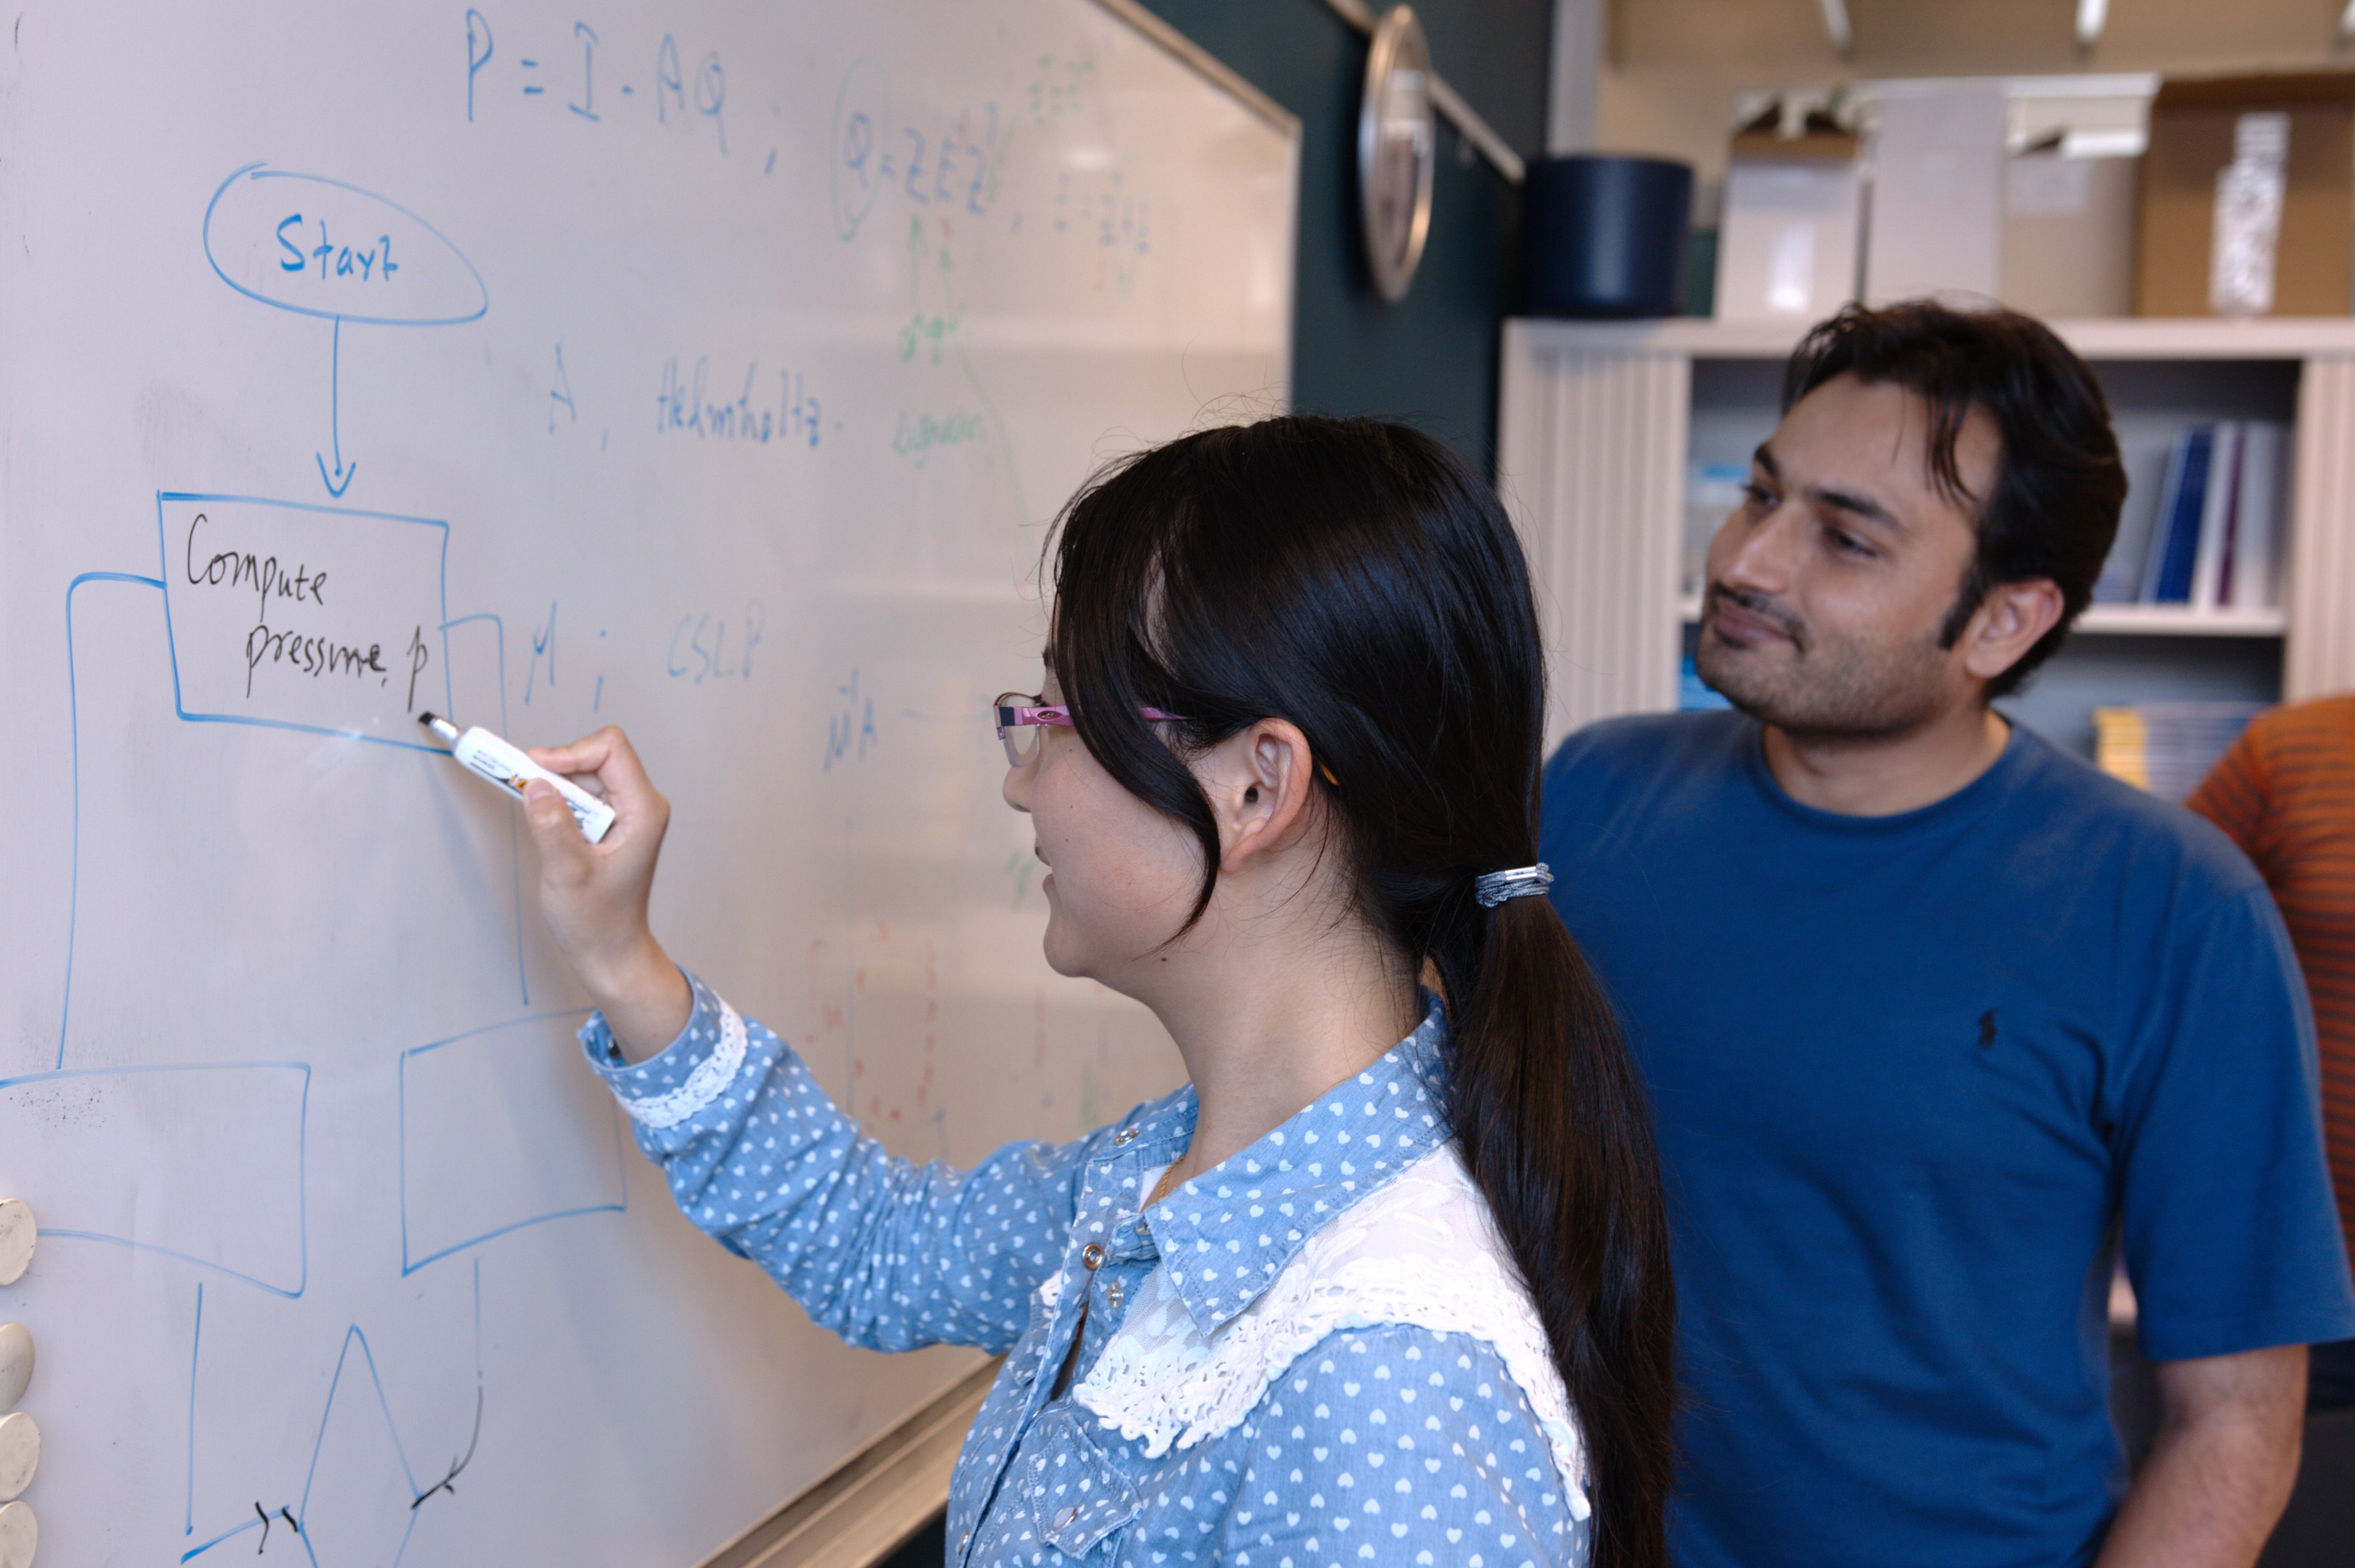
\includegraphics[width=0.75\textwidth]{images/whiteboard1}
  \end{figure}
 \end{column}
 \end{columns}
\end{frame}

\begin{frame}
\frametitle{Who are we?}
\begin{figure}
 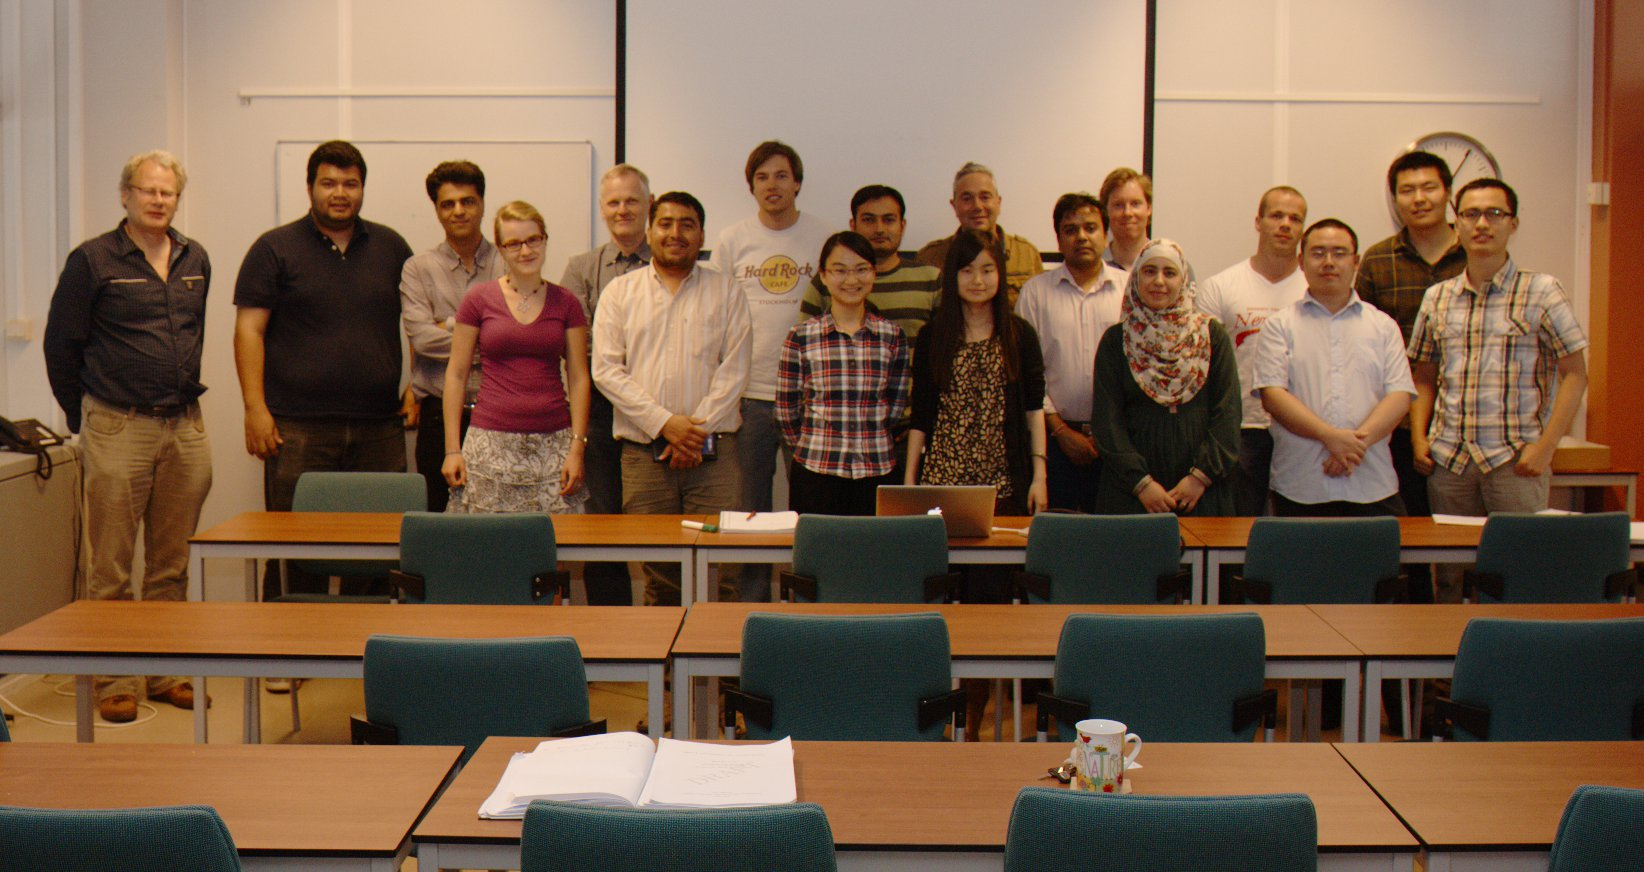
\includegraphics[width=\textwidth]{images/group}
\end{figure}
\end{frame}

\begin{frame}
   The Chapter at TU Delft has been {\color{blue}founded in 2014}.
  \vspace{-0.3cm}
  \begin{itemize}
    \item {\color{blue}P:} Manuel Baumann
    \item {\color{blue}VP:} Reinaldo Astudillo
    \item {\color{blue}Sec. \& Treas.:} Thea Vuik
    \item ... and many more ;-)
  \end{itemize}

  Our faculty advisors are:
  \vspace{-0.3cm}
  \begin{itemize}
    \item Kees Vuik
    \item Martin van Gijzen
  \end{itemize}

  The Chapter is {\color{blue}open} for MSc and PhD students as well as staff members.
\end{frame}


\begin{frame}
\frametitle{What happened so far?}
\begin{columns}
 \begin{column}{0.8\textwidth}
 \begin{itemize}
  \item Students from Numerical Analysis started the so-called ``Project ba{\color{red}NaN}a'':
  \begin{itemize}
  \item learning-by-doing sessions
  \item focus on software tools like \texttt{git}, \texttt{JabRef}, ...
  \item have bananas together after work
 \end{itemize}
 \item Tea talks
 \item Some social events (bowling, BBQ, ...)
 \end{itemize}
 \end{column}

 \begin{column}{0.4\textwidth}
  \begin{figure}[t]
  \centering
  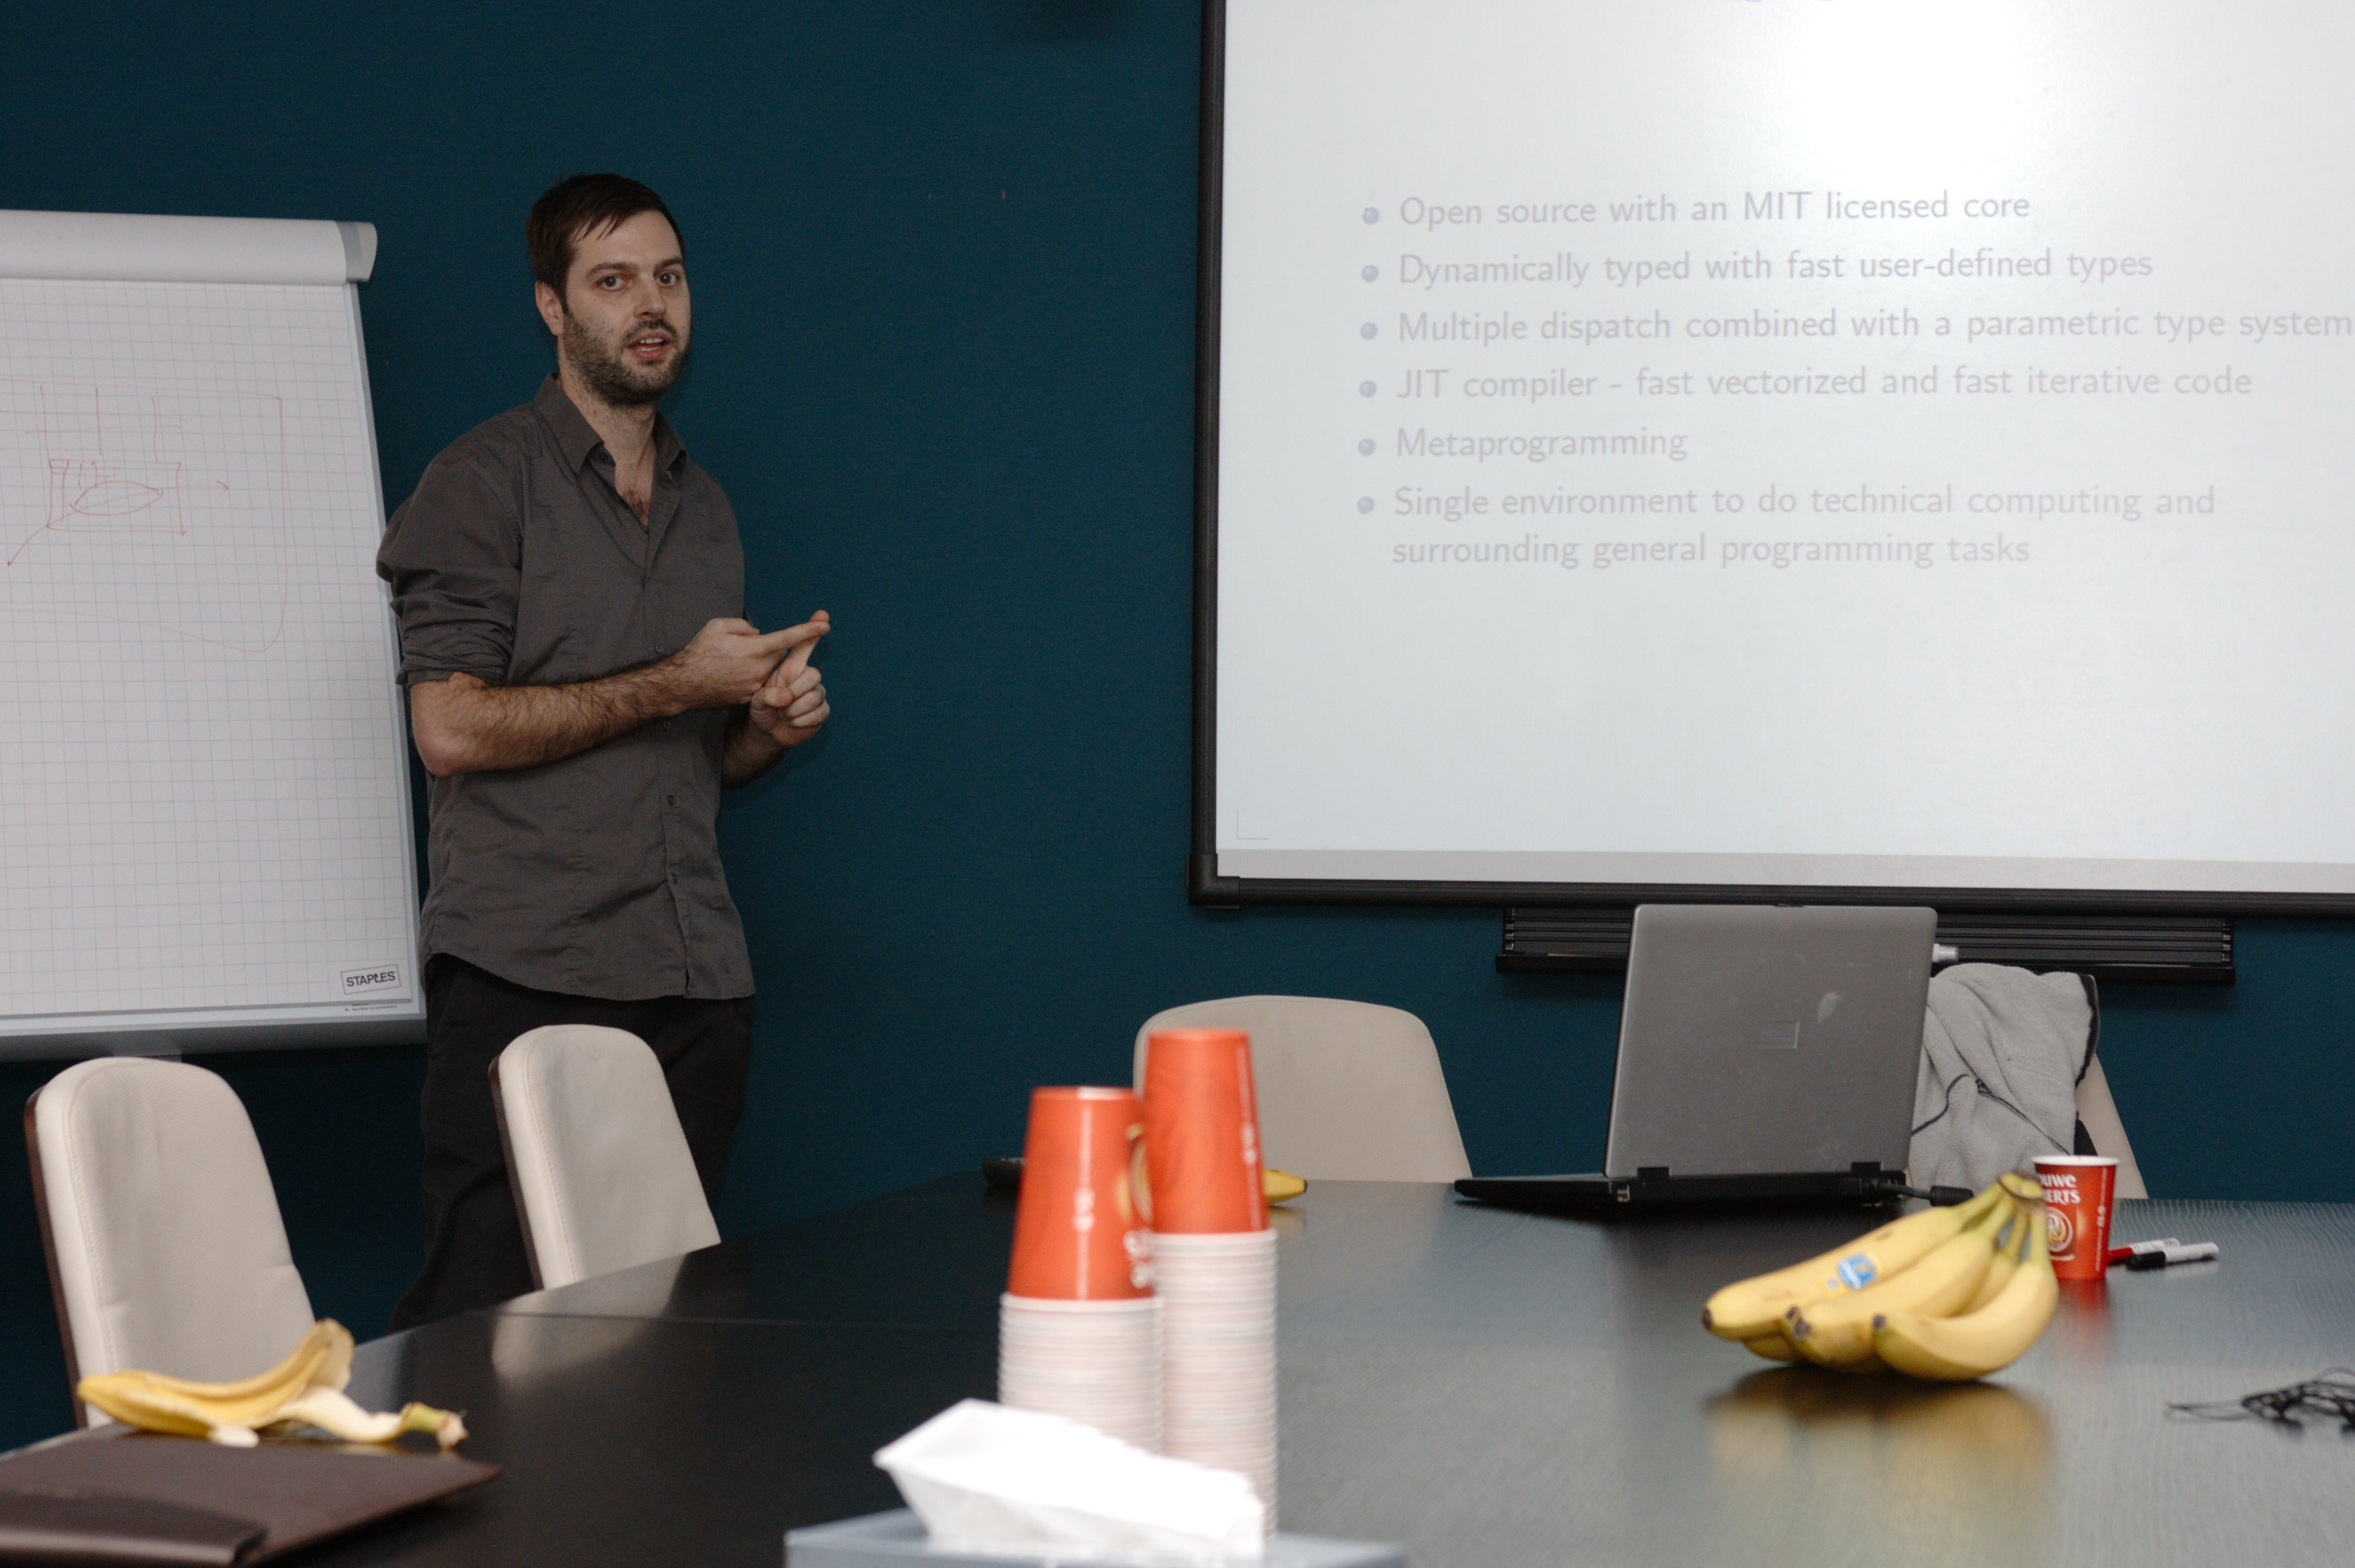
\includegraphics[width=0.8\textwidth]{images/moritz} \vspace{0.6cm}\\
  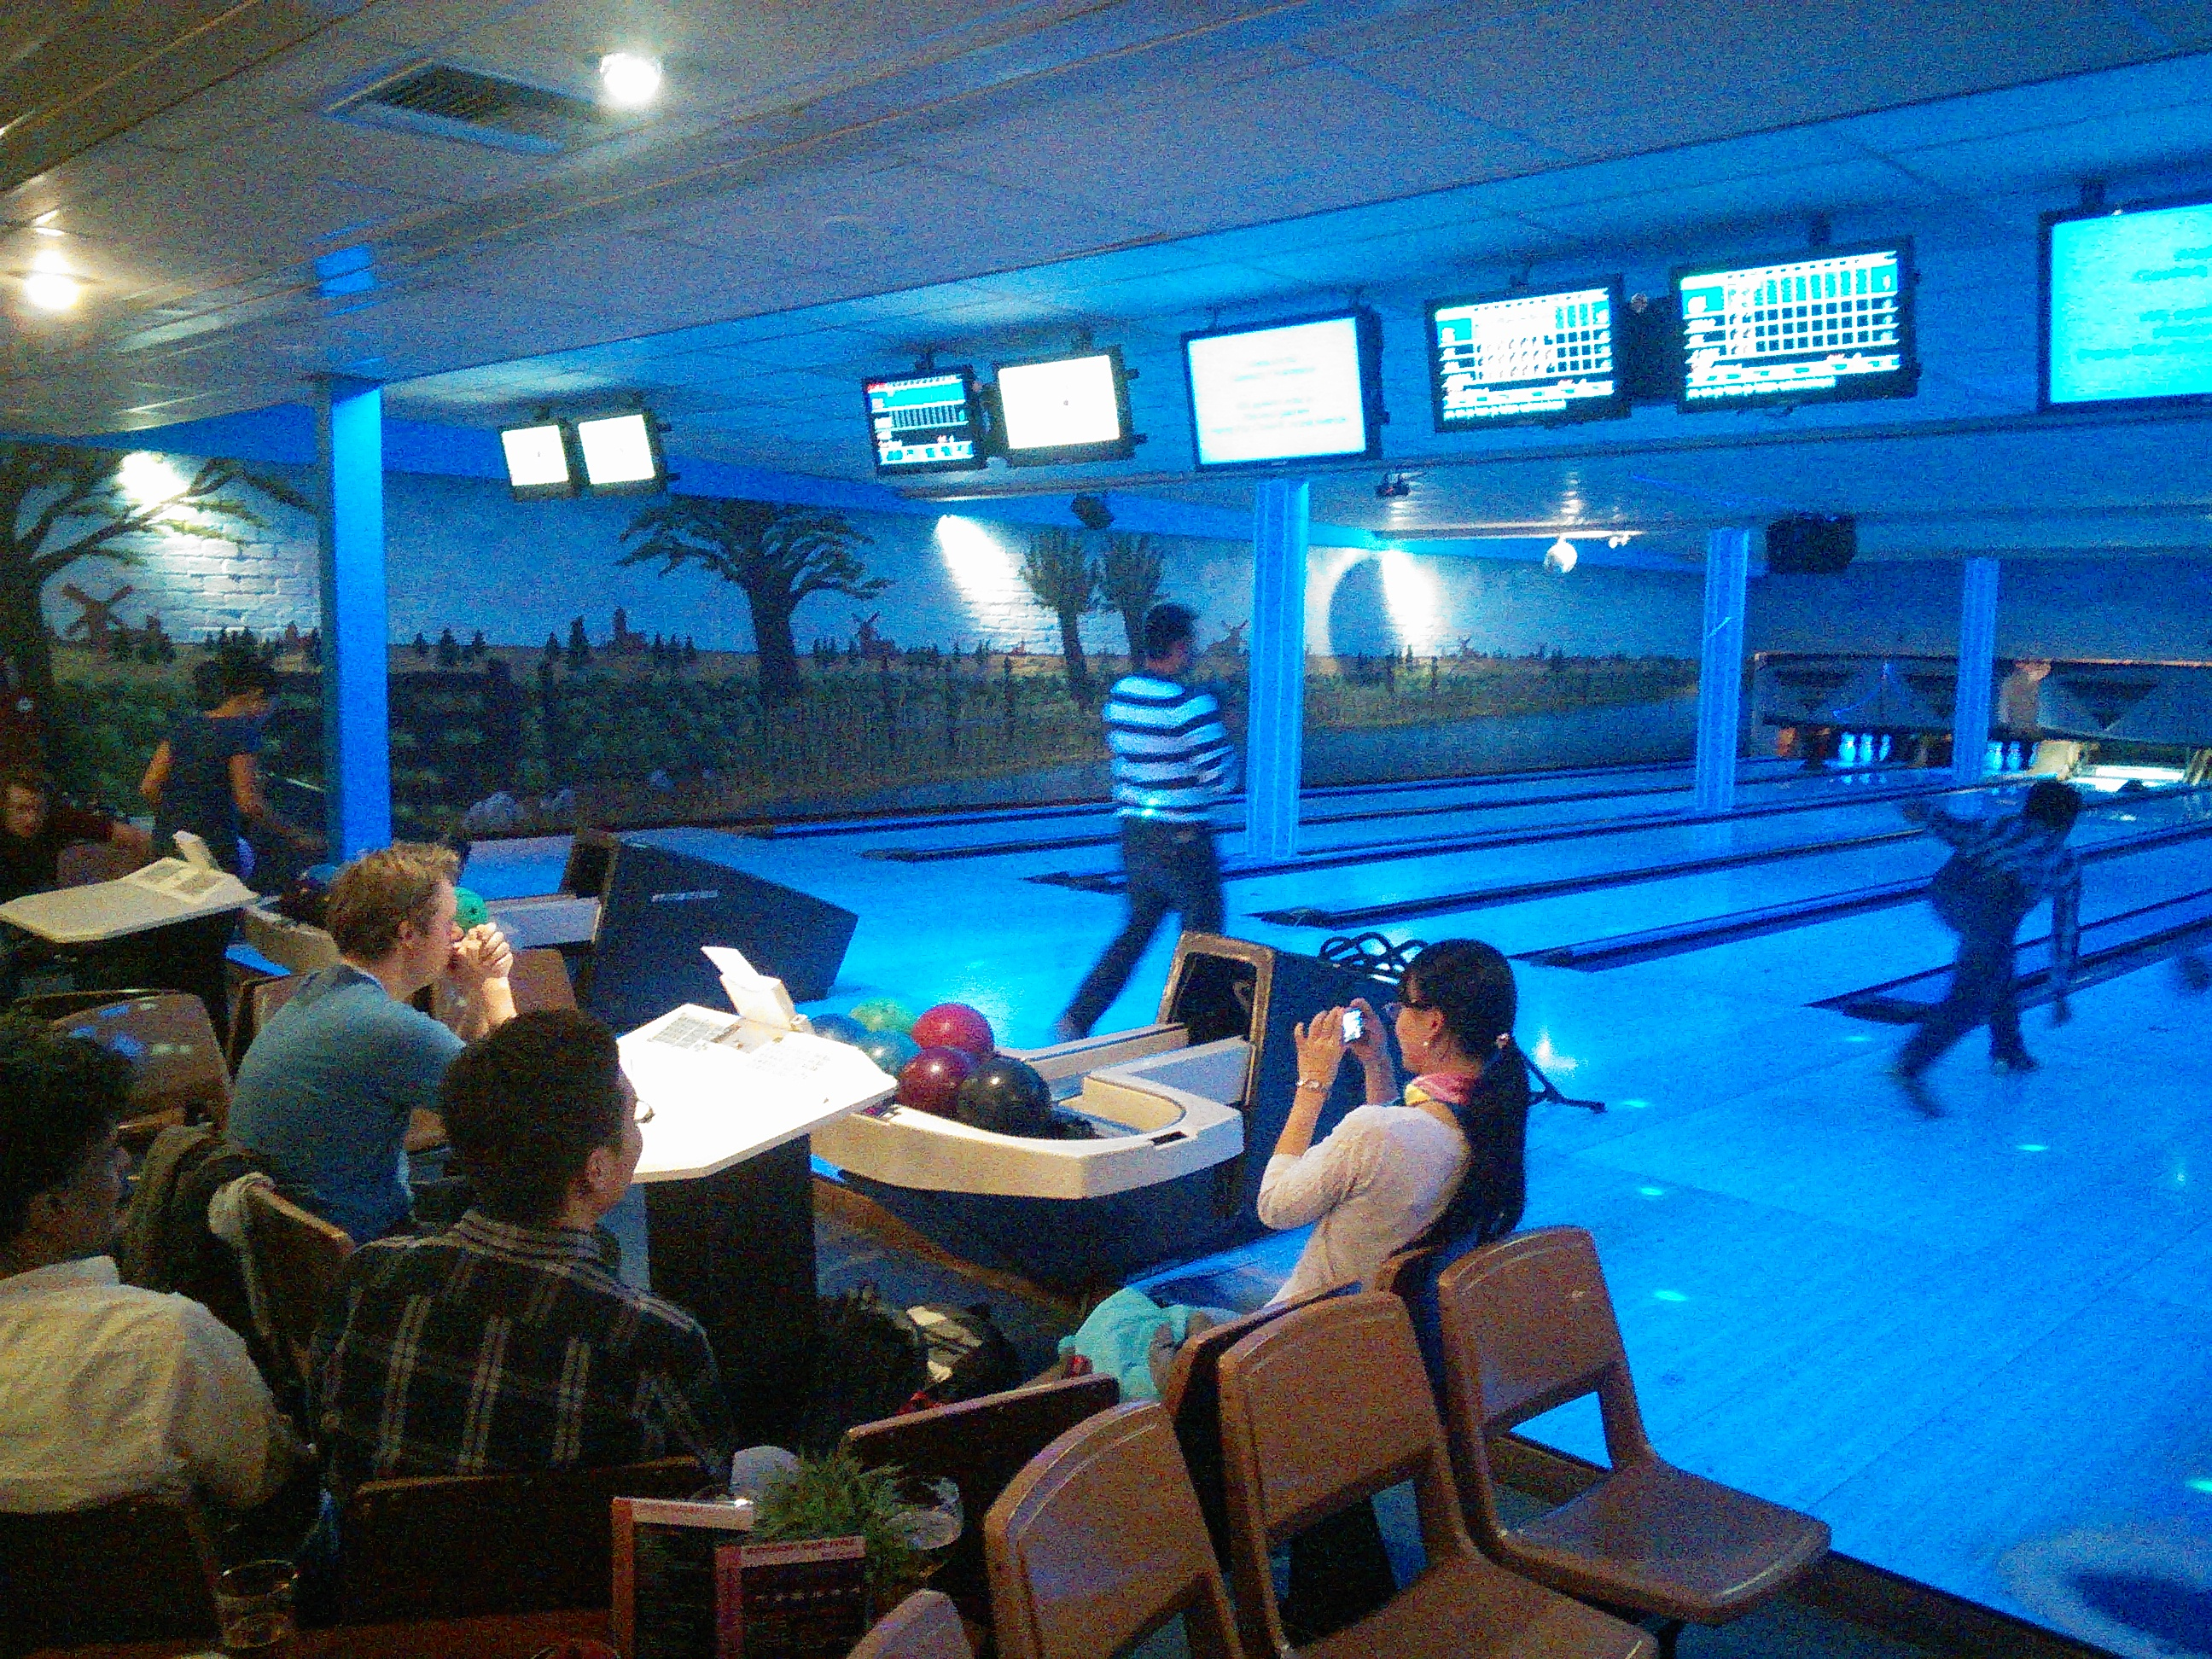
\includegraphics[width=0.8\textwidth]{images/bowling}
  \end{figure}
 \end{column}
 \end{columns}
\end{frame}

\begin{frame}
\frametitle{Future activities}
\begin{columns}
 \begin{column}{0.8\textwidth}
 \begin{itemize}
  \item Student Krylov day at TU Delft on February 2nd, 2015
  \item more ba{\color{red}NaN}a talks:
  \begin{itemize}
      \item Python
      \item Paraview
      \item Latex
      \item ...
  \end{itemize}
  \item company visits:
    \begin{itemize}
      \item data steel
      \item Deltares
      \item VORtech
  \end{itemize}
 \end{itemize}

 \end{column}

 \begin{column}{0.4\textwidth}
  \begin{figure}[t]
  \centering
  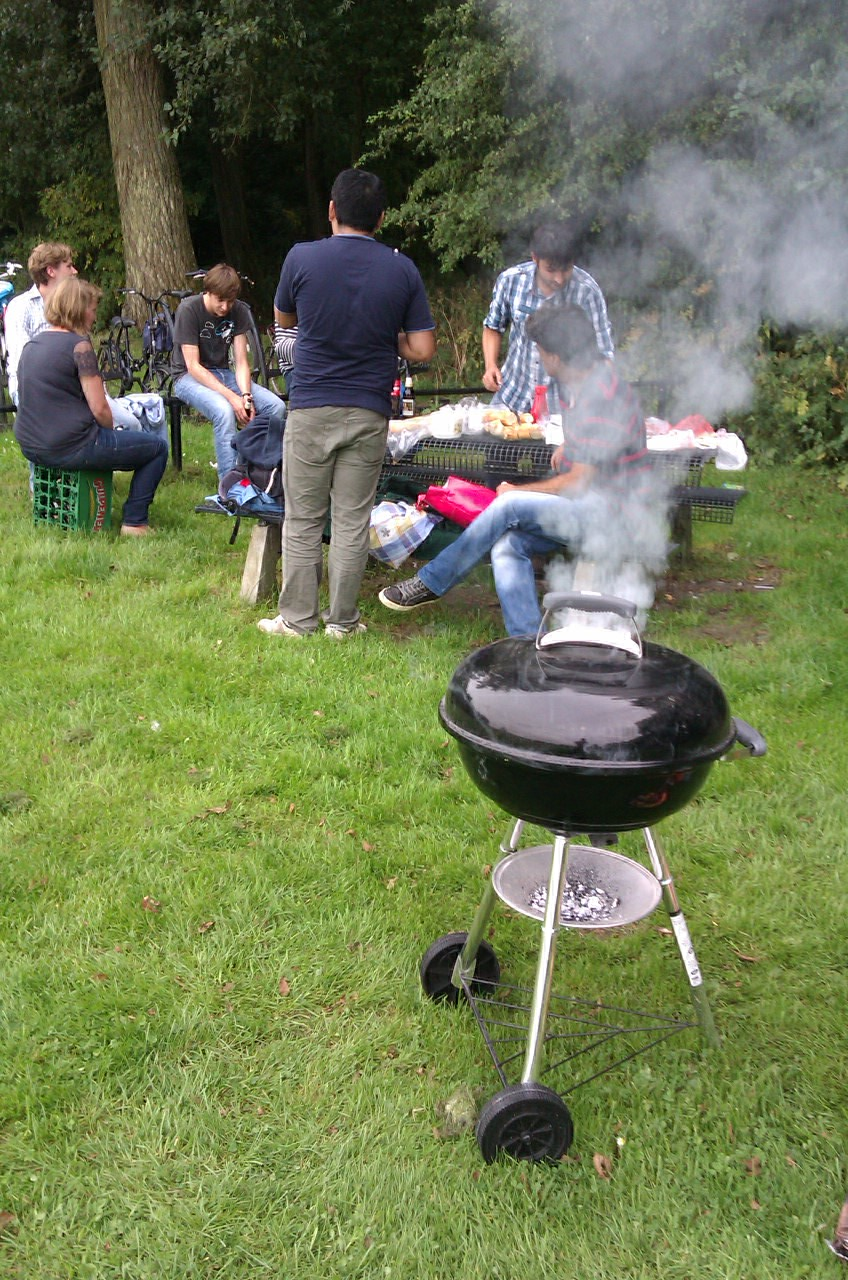
\includegraphics[width=0.8\textwidth]{images/bbq}
  \end{figure}
 \end{column}
 \end{columns}
\end{frame}

\begin{frame}
\frametitle{How to get in touch?}
There are many ways to get in touch with us:
\begin{itemize}
 \item Twitter: \href{https://twitter.com/SSC\_Delft}{@SSC\_Delft}
 \item email: siamsc-ewi@tudelft.nl
 \item homepage: \href{http://sscdelft.github.io}{http://sscdelft.github.io}
 \item sign in the member list
\end{itemize}
\begin{figure}[t]
\hfill
\includegraphics[scale=0.14]{SSC_Delft_new}
\end{figure}
\end{frame}

\begin{frame}
\frametitle{Today's schedule}
\begin{description}[scheduleoftoday]
 \item[16:00 - 16:10] Introduction
 \item[16:10 - 16:35] Kees Vuik - mathematical modelling
 \item[16:35 - 17:00] Alex Sangers - google PakeRank
 \item[after 17:00] cake and get-together
\end{description}
\end{frame}
\end{document}
